\documentclass[11pt, a4paper]{article}

\usepackage{graphicx}
\usepackage[a4paper,top=3cm,bottom=2cm,left=2cm,right=2cm,marginparwidth=1.75cm]{geometry}
\usepackage[english]{babel}
\usepackage[utf8x]{inputenc}
\usepackage{subfig}
\usepackage{float}
\usepackage{amsmath}
\usepackage{amssymb}
\usepackage{mhchem}


\graphicspath{ {./images} }
\newcommand*{\qed}{\hfill\ensuremath{\quad\square}}
\newcommand*{\rad}{\ensuremath{\,\text{rad}}}
\newcommand*{\R}{\ensuremath{\mathbb{R}}}

\makeatletter
\renewcommand*\env@matrix[1][*\c@MaxMatrixCols c]{%
  \hskip -\arraycolsep
  \let\@ifnextchar\new@ifnextchar
  \array{#1}}
\makeatother

\newtheorem{theorem}{Theorem}

%------------------------------------------------
%Templates for images and figures
% \begin{figure}[h]
%   \centering
%   \subfloat[caption 1]{{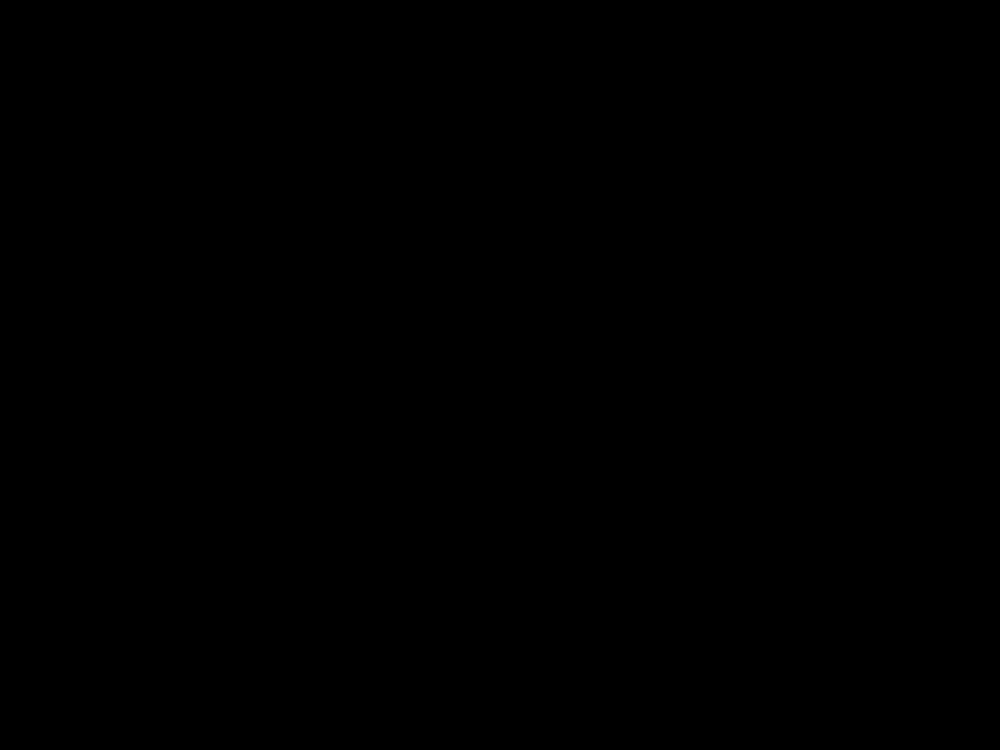
\includegraphics[width=30mm]{images/placeholder.png}}}%
%   \qquad
%   \subfloat[caption 2]{{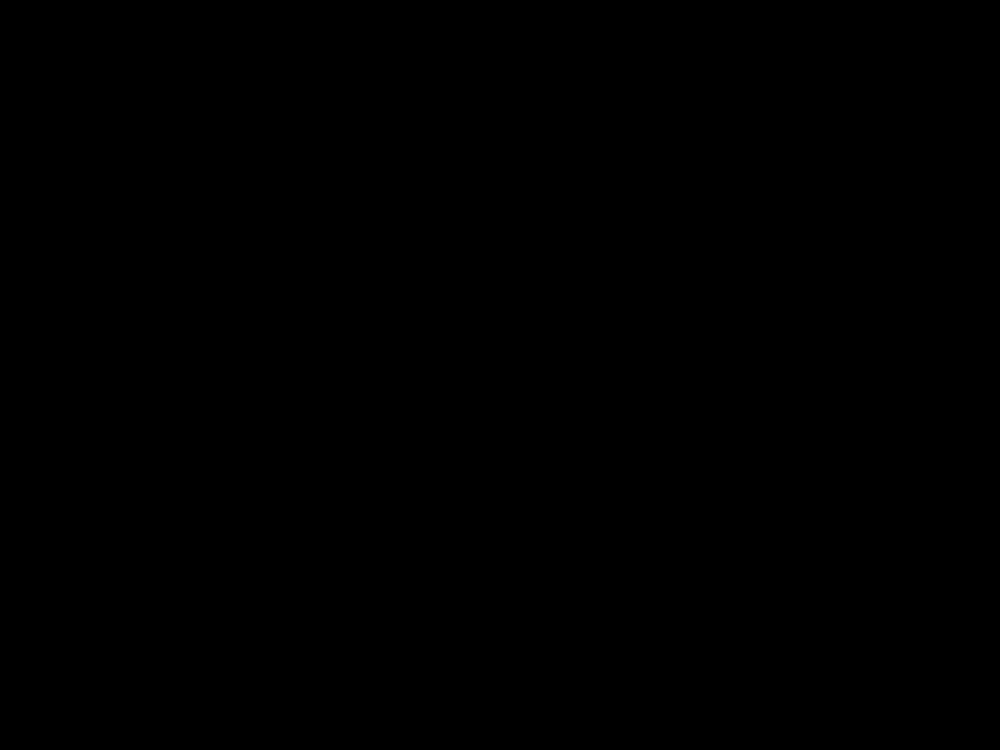
\includegraphics[width=30mm]{images/placeholder.png}}}%
%   \caption{Description}
% \end{figure}

% \begin{figure}[h]
%   \centerline{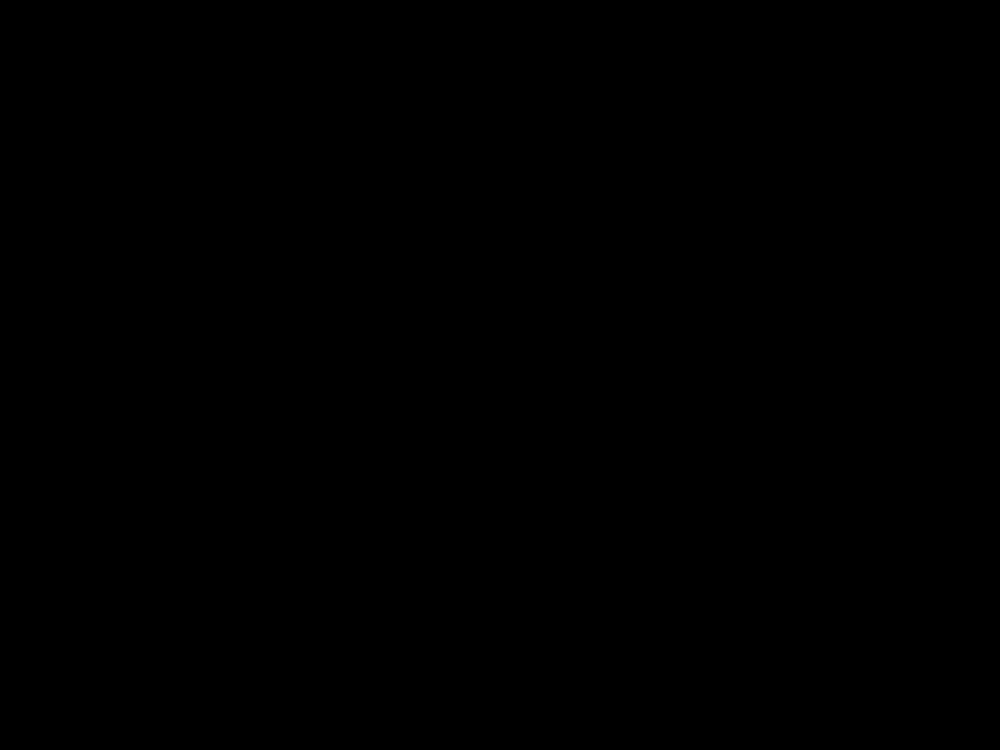
\includegraphics[width=50mm]{images/placeholder.png}}
%   \caption{Description}
% \end{figure}

%Template for a simple table 
%\begin{table}[h]
%   \caption{Description} %title of the table
%   \centering % centering table
%   \begin{tabular}{l rr} % creating three columns
%     \hline\hline %inserting double-line
%     & & \\ [0.5ex] % Insert half line vertical spacing
%     \hline % inserts single-line
%     & & \\ 
%     & & \\
%     & & \\
%     & & \\
%   \hline % inserts single-line
%   \end{tabular}
%   \label{tab:hresult}
% \end{table}
%-----------------------------------------------

\begin{document}
\setcounter{equation}{0}
\setcounter{section}{3}

\section{WOP3B Lecture 4: Fatigue (07/05/2020)}


\subsection{Defining fatigue}
Fatigue refers to the weakening or even failure of a material caused by cyclical loading. It usually results in localized damage to parts or structures such as cracks. Fatigue can be prevented by designing larger, heavier parts, however due to material costs, logistical complications and overall efficiency of machines this is not the preferable solution. Downsizing and weight-saving is very important in many fields of engineering, such as robotics, automotive design, machine design and areo-space since there is a direct relation between mass and energy consumption. Thus more mass directly implies more energy required. In the case of shooting a rocket into space it's easy to see why this is a problem. Making parts less stiff and more fragile does however bring problems with it, such as lower fatigue life.


\subsection{Low cycle fatigue}
In cases where parts undergo large strains (deformations) due to either mechanical, thermal or thermo-mechanical reasons (e.g. semi-conductors and the plastic buckle clip things) we analyze the strain life relationship (e$N$-curve or $\epsilon N$-curve) of the part. This curve shows the relation between strain $\Delta \epsilon$ and the amount of cycles $N$. Large deformation usually lead to a relativly short life cylce (in the range of $1000-10.000$ cycles). Hence the name LCF (Low Cycle Fatigue).
\begin{figure}[h]
  \centerline{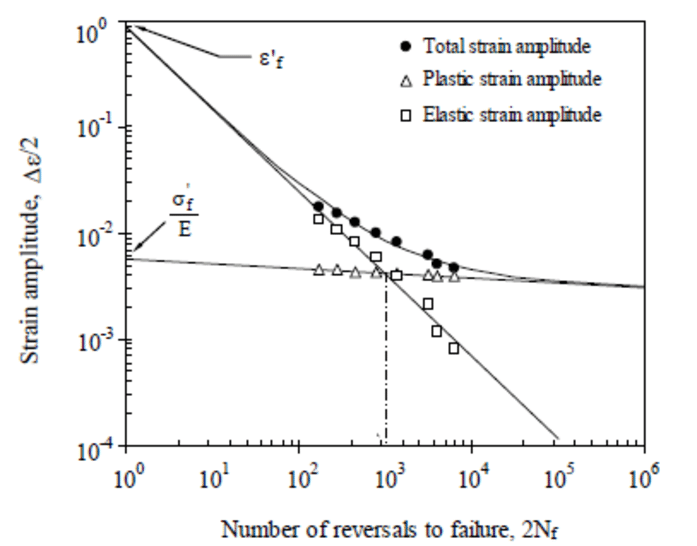
\includegraphics[width=80mm]{images/eN_curve.png}}
  \caption{An example of an $\epsilon N$-curve}
  \label{fig:eN}
\end{figure}


\subsection{High Cycle Fatigue}
Some parts may undergo large cyclical stresses. An example of such a part is an axle in a vehicle. In cases like these we instead look at the stress life relationship ($SN$-curve). The number of cycles will always be way larger then $10^4$, hence the name HCF (High Cycle Fatigue).
\begin{figure}[h]
  \centerline{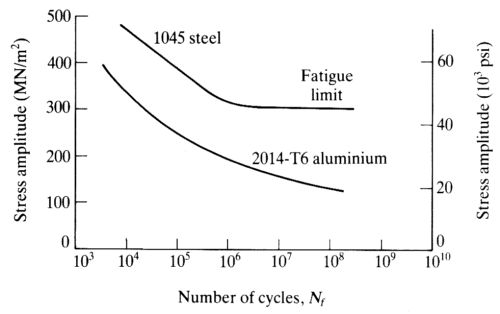
\includegraphics[width=80mm]{images/SN_curve.jpg}}
  \caption{An example of an $SN$-curve}
  \label{fig:SN}
\end{figure}

\subsection{Endurance limit}
Ferrous alloys and titanium show what is referred to as an endurance limit. This means that any stresses which are below a given value $\Delta \sigma_e$ will not fail no matter the amount of cycles. Most other structural metals such as \ce{Al}, \ce{Cu}, \ce{Mg}, \ce{Ni}-alloys, some stainless steels and high alloy steels do not have an endurance limit. This means that the material will always fail when $N$ becomes sufficiently large, even under low stress. In these cases the fatigue strength is usually listed for $10^7$ cycles. In case of finite life stresses below $\Delta \sigma_e$ are referred to as safe life design. A visual example of an endurance limit as it would be seen in an $SN$-curve can be found in figure \ref{fig:SN}


\subsection{Palmgren-Miner rule}
Usually when doing field tests with a strain gauge the result will not be a clean graph. To translate this graph into a more usable data set we look at the peaks in stress $\Delta \sigma$ and count how many times these occur. We then plot those in a histogram. This process is referred to as rain-flow counting.
\begin{figure}[h]
  \centering
  \subfloat[The stress graph]{{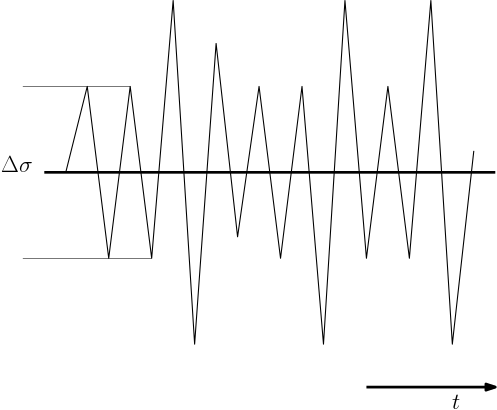
\includegraphics[width=60mm]{images/Stress_gauge.png}}}%
  \qquad \qquad
  \subfloat[The resulting histogram]{{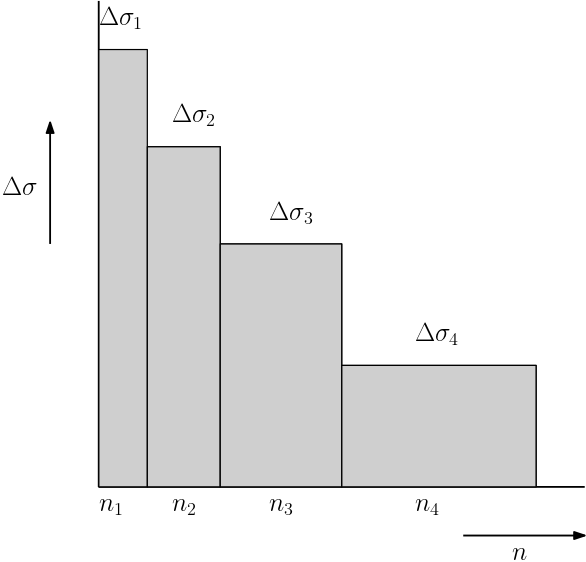
\includegraphics[width=60mm]{images/Histogram.png}}}%
  \caption{Visualization of the rain-flow counting process where (a) is the graph from some stress gauge and (b) is the resulting histogram.}
  \label{fig:RFC}
\end{figure}
The histogram is then visualized on an $SN$-curve of the corresponding material. An example of this is shown in figure \ref{fig:SN2}. When looking at this figure the load $\Delta \sigma_1$ was applied $n_1$ times. The amount of cycles this load would need to be applied before failure occurs corresponds to $N_1$. The part of the life cycle that was used by $\Delta \sigma_1$ can then be expressed as $\frac{n_1}{N_1}$. The total fraction of the life cycle used then becomes the summation of all the individual damage fractions:
\begin{equation}
  D = \sum_{i=1}^{k} \frac{n_i}{N_i}
\end{equation}
The expected life cycle then becomes:
\begin{equation}
  L = \frac{T}{D}
\end{equation}
Where $T$ is the time tested and $D$ is the earlier defined total damage fraction. It's interesting to note that larger stresses have a disproportianally large effect on the total damage fraction. Thus when doing any type of fatigue testing the process can be accelrated considerably by applying a larger stress.
\begin{figure}[H]
  \centerline{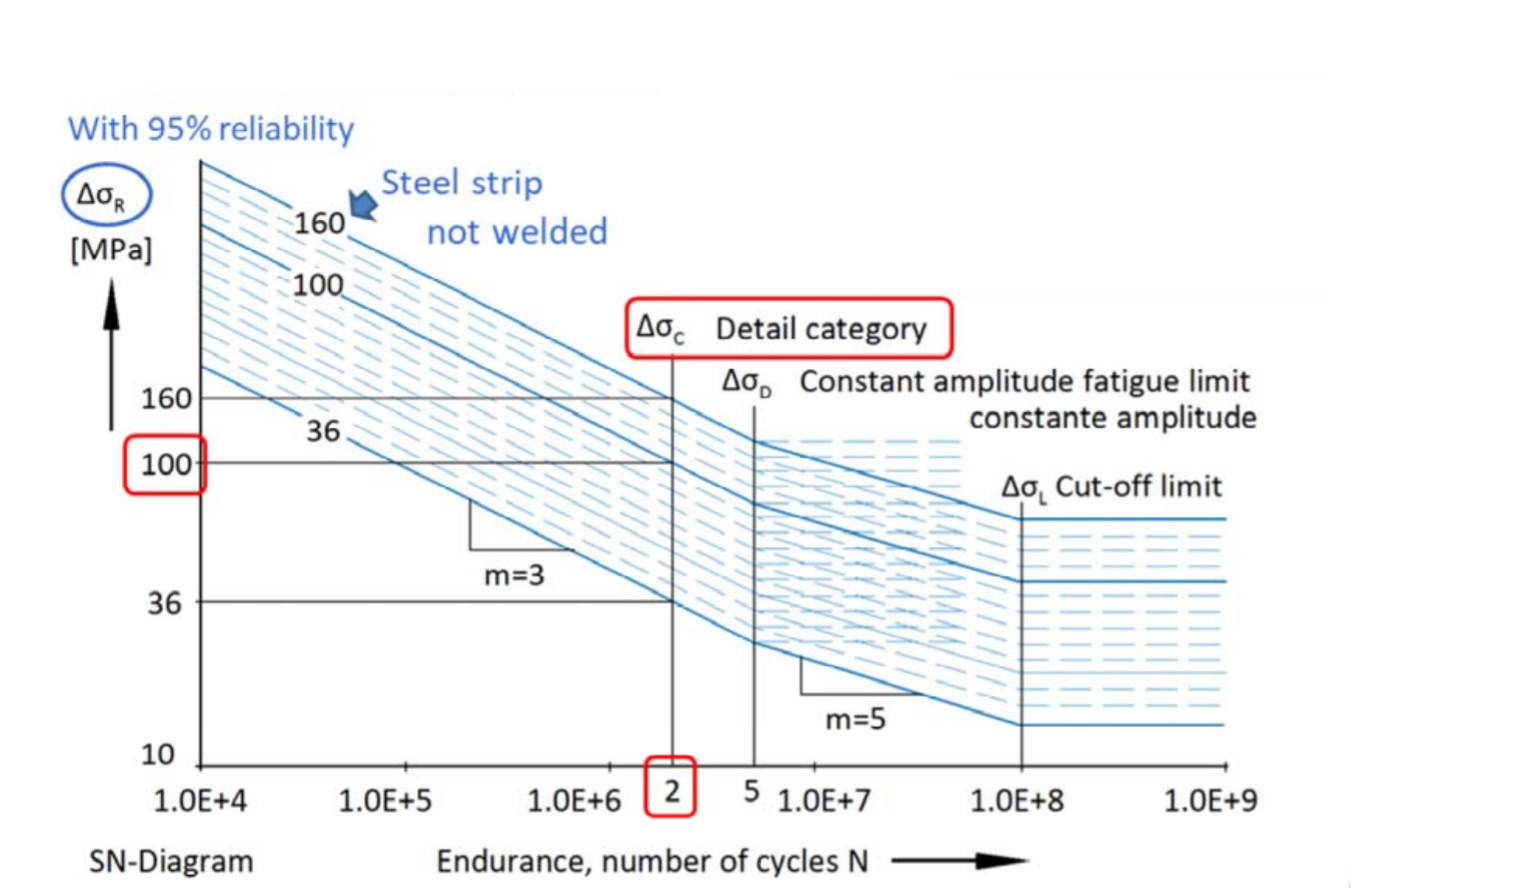
\includegraphics[width=80mm]{images/SN_curve.png}}
  \caption{The data from the histogram plotted in the corresponding $SN$-curve}
  \label{fig:SN2}
\end{figure}


\end{document}